\begin{figure}[H]
    \centering
    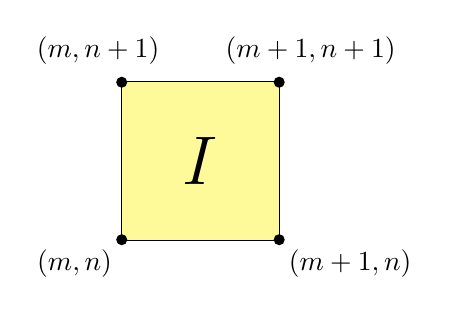
\begin{tikzpicture}
  
    \draw[thick] (0,0) -- (2,0) -- (2,2) -- (0,2) -- cycle;
    \fill[yellow!40] (0,0) rectangle (2,2);
    
    \fill (0, 0) circle (2pt);  
    \fill (2, 0) circle (2pt);  
    \fill (2, 2) circle (2pt); 
    \fill (0, 2) circle (2pt);  

    \node[below left] at (0, 0) {$(m, n)$};
    \node[below right] at (2, 0) {$(m+1, n)$};
    \node at (2.4, 2.4) {$(m+1, n+1)$};
    \node at (-0.3, 2.4) {$(m, n+1)$};

    \node at (1, 1) {\Huge $I$};
    
    
\end{tikzpicture}
    \caption{A $2$-cube $I$}
    \label{fig_2_cube}
\end{figure}